\RequirePackage{amsthm} %https://tex.stackexchange.com/questions/687324/unknown-theoremstyle-warning-with-springer-nature-template
\documentclass[sn-mathphys-num,icol]{sn-jnl}
%\documentclass[sn-mathphys-num,iicol]{jnl}

%\usepackage{sn-jnl.sty}
\usepackage[pscoord]{eso-pic}% The zero point of the coordinate systemis the lower left corner of the page (the default).

\usepackage[absolute,overlay]{textpos}
\usepackage[dvipsnames]{xcolor}
\usepackage{tikz}
\usepackage{graphicx}% \usepackage{multirow}% \usepackage{cuted}
\usepackage{amsmath,amssymb,amsfonts}%
\usepackage{amsthm}%
\usepackage{gensymb}
\usepackage{physics}
\usepackage[locale=US]{siunitx}
\usepackage{mathrsfs}%
\usepackage[title]{appendix}%
\usepackage{xcolor}%
\usepackage{textcomp}%
\usepackage{manyfoot}%
\usepackage{booktabs}%
\usepackage{algorithm}%
\usepackage{algorithmicx}%
\usepackage{algpseudocode}%
\usepackage{listings}%
\usepackage{newtxmath}%
\usepackage{yfonts}
\usepackage{braket}
\usepackage{dsfont}
\usepackage{subfig}
\usepackage[tiny]{titlesec}%
\usepackage[american]{babel}
\usepackage{cleveref}

\usetikzlibrary{arrows.meta, positioning, shapes.geometric, decorations.markings}

\theoremstyle{thmstyleone}
\newtheorem{theorem}{Theorem}
\newtheorem{proposition}[theorem]{Proposition}

\theoremstyle{thmstyletwo}
\newtheorem{remark}{Remark}

\theoremstyle{thmstylethree}
\newtheorem{definition}{Definition}

\raggedbottom

\newcommand{\td}{\text{d}}

\titleformat{\subsection}{}{\thesubsection}{1em}{\itshape}
\titleformat{\subsubsection}{}{\thesubsubsection}{1em}{\itshape}

\begin{document}

\title{K223: Nuclear $\gamma\gamma$ Angular Correlations}
\author*[1]{\fnm{Dhruv} \sur{Pisharody}}\email{}
\author*[1]{\fnm{Angelo} \sur{Brade}}\email{s72abrad@uni-bonn.de}
\affil*[1]{Rheinische Friedrich--Wilhelms--Universität, Bonn}
\maketitle
\section{Analysis of the Data}
\subsection{Calibration of the SCAs}

\begin{figure}[H]
	\begin{center}
		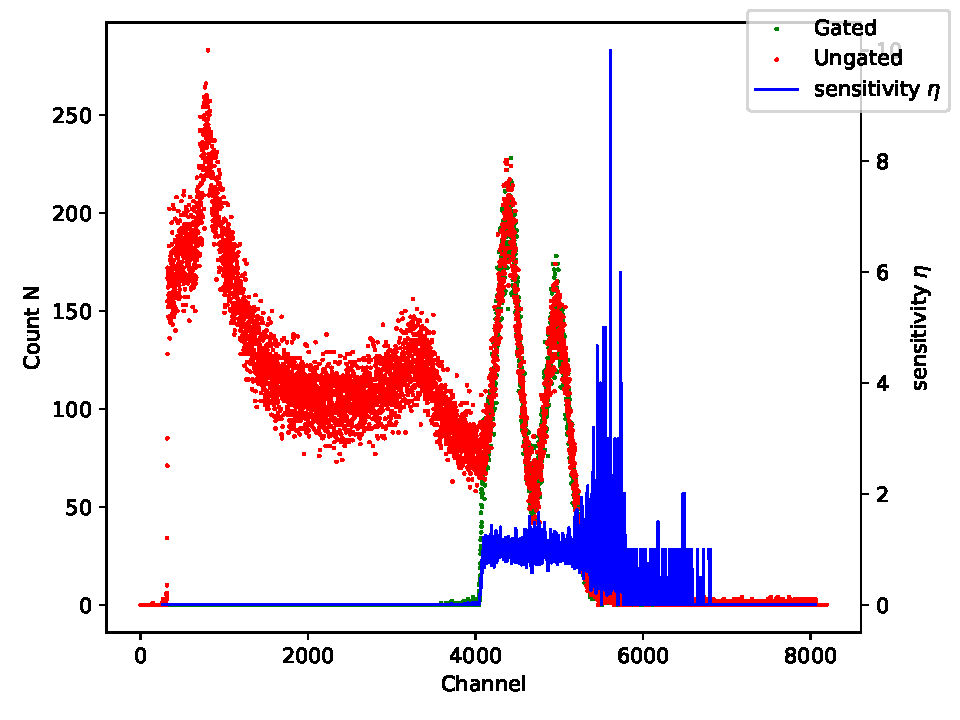
\includegraphics[width=1\textwidth]{../images/SCA_Calib_C.pdf}
	\end{center}
	\caption{SCA Spectrum for Stationary Detector}\label{fig:sca_calib_c}
\end{figure}

\begin{figure}[H]
	\begin{center}
		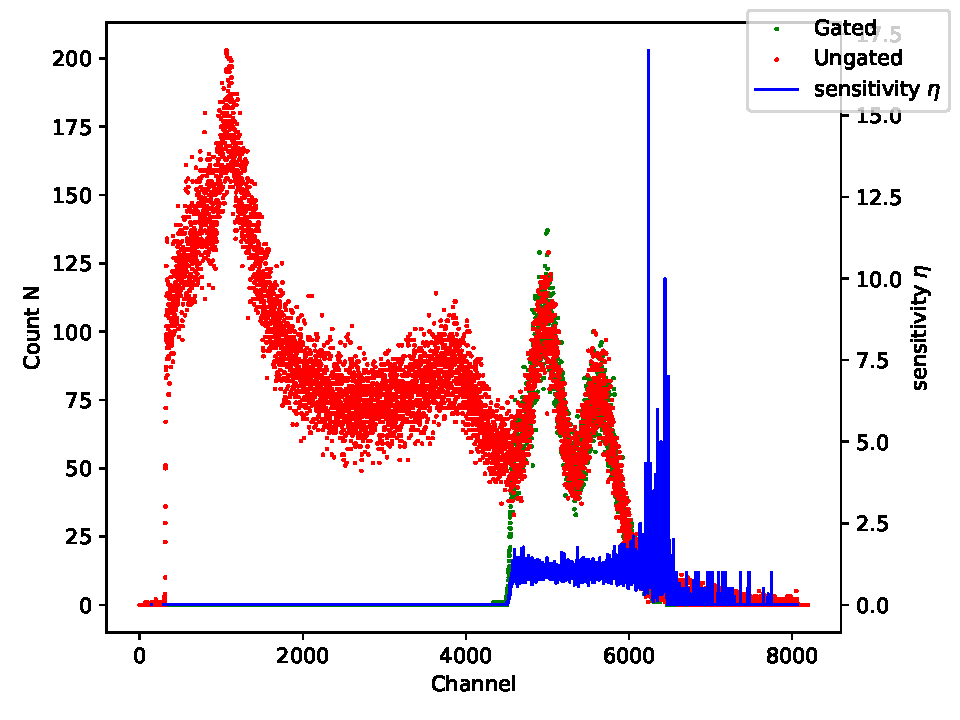
\includegraphics[width=1\textwidth]{../images/SCA_Calib_M.pdf}
	\end{center}
	\caption{SCA Spectrum for Moving Detector}\label{fig:sca_calib_m}
\end{figure}

\begin{figure}[H]
	\begin{center}
		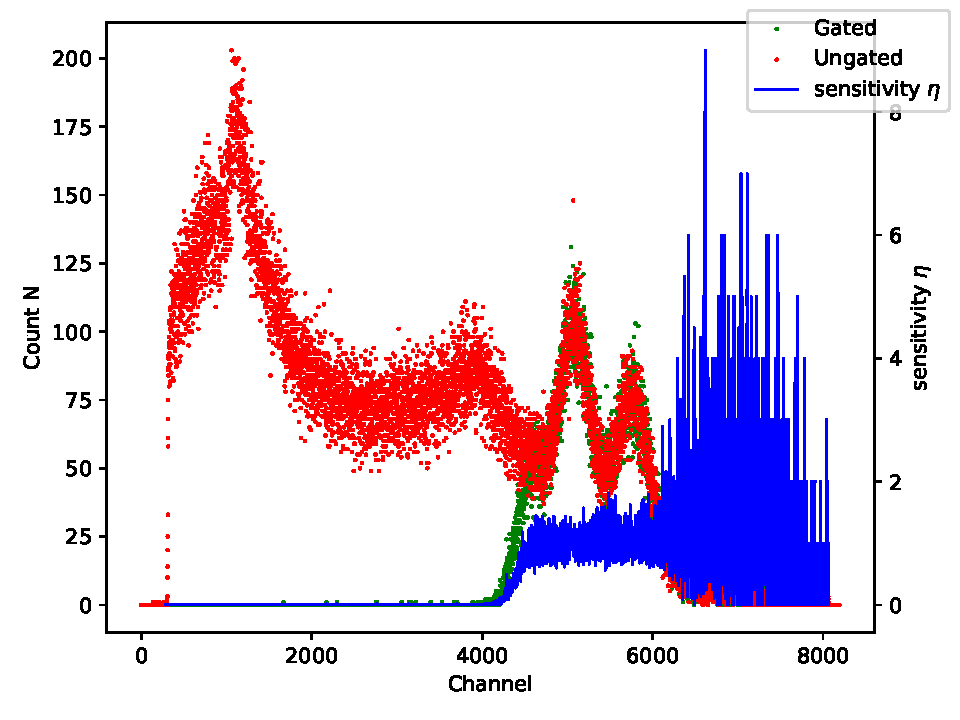
\includegraphics[width=1\textwidth]{../images/CFD_Calib_C.pdf}
	\end{center}
	\caption{CFD Spectrum for Stationary Detector}\label{fig:sca_calib_c}
\end{figure}

\begin{figure}[H]
	\begin{center}
		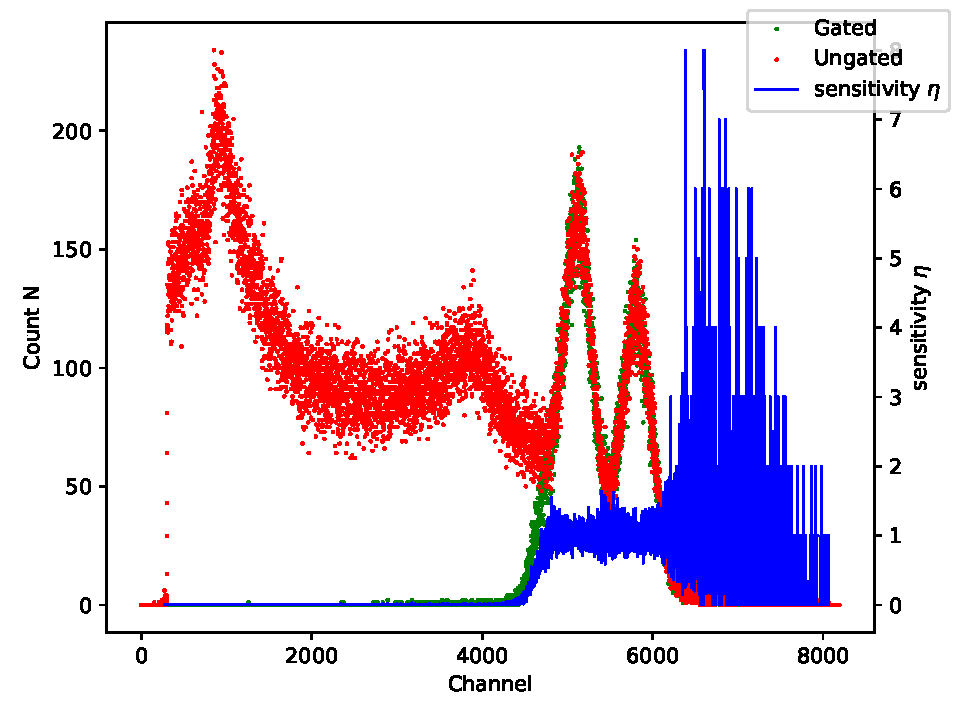
\includegraphics[width=1\textwidth]{../images/CFD_Calib_M.pdf}
	\end{center}
	\caption{CFD Spectrum for Moving Detector}\label{fig:sca_calib_m}
\end{figure}

\begin{figure}[H]
	\begin{center}
		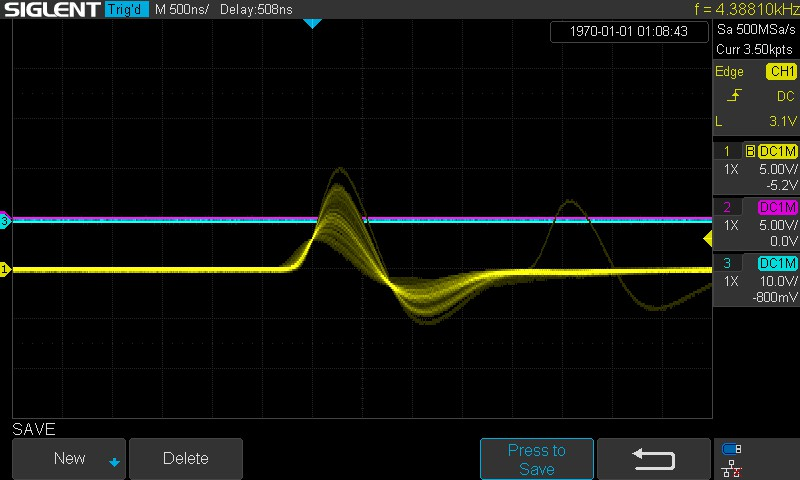
\includegraphics[width=1\textwidth]{../images/SDS00001.jpg}
	\end{center}
	\caption{CFD Spectrum for Moving Detector}\label{fig:sca_calib_m}
\end{figure}
\begin{figure}[H]
	\begin{center}
		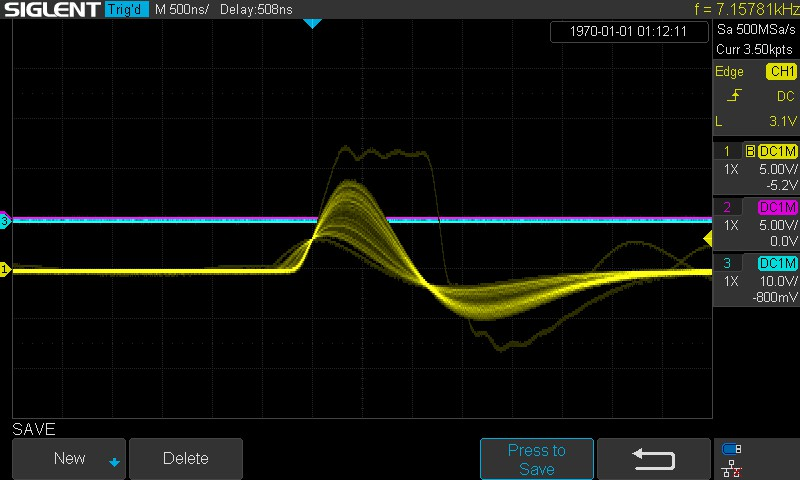
\includegraphics[width=1\textwidth]{../images/SDS00002.jpg}
	\end{center}
	\caption{CFD Spectrum for Moving Detector}\label{fig:sca_calib_m}
\end{figure}
\begin{figure}[H]
	\begin{center}
		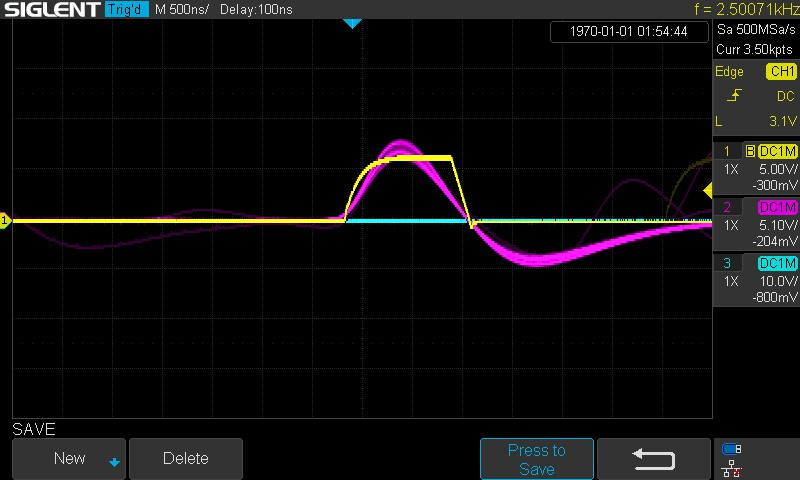
\includegraphics[width=1\textwidth]{../images/SDS00003.jpg}
	\end{center}
	\caption{CFD Spectrum for Moving Detector}\label{fig:sca_calib_m}
\end{figure}
\begin{figure}[H]
	\begin{center}
		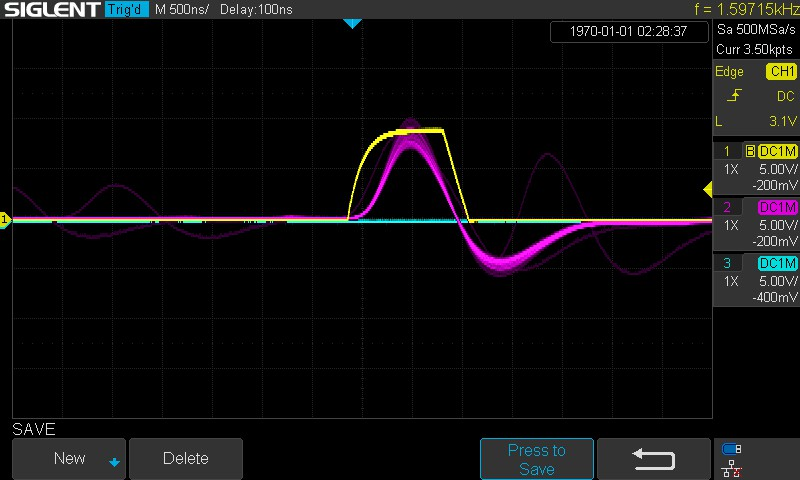
\includegraphics[width=1\textwidth]{../images/SDS00004.jpg}
	\end{center}
	\caption{CFD Spectrum for Moving Detector}\label{fig:sca_calib_m}
\end{figure}
\begin{figure}[H]
	\begin{center}
		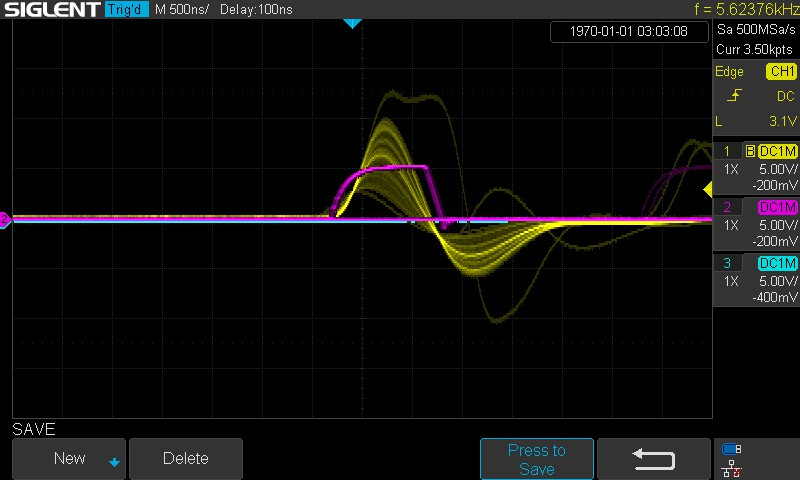
\includegraphics[width=1\textwidth]{../images/SDS00005.jpg}
	\end{center}
	\caption{CFD Spectrum for Moving Detector}\label{fig:sca_calib_m}
\end{figure}
\begin{figure}[H]
	\begin{center}
		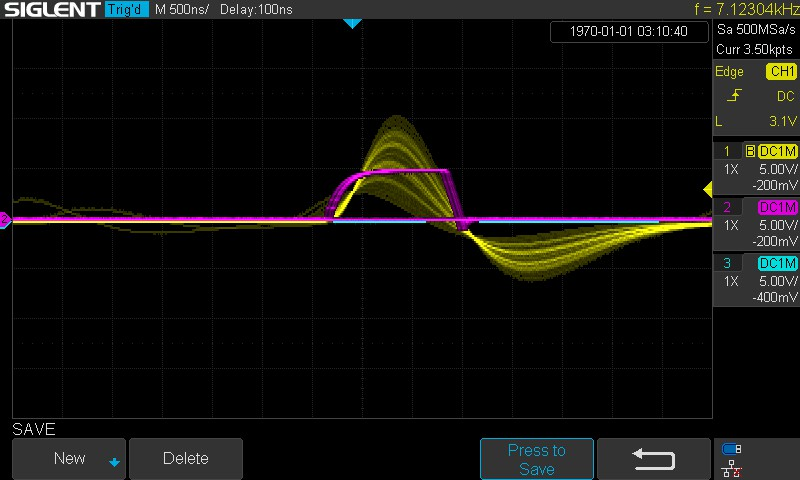
\includegraphics[width=1\textwidth]{../images/SDS00006.jpg}
	\end{center}
	\caption{CFD Spectrum for Moving Detector}\label{fig:sca_calib_m}
\end{figure}
\begin{figure}[H]
	\begin{center}
		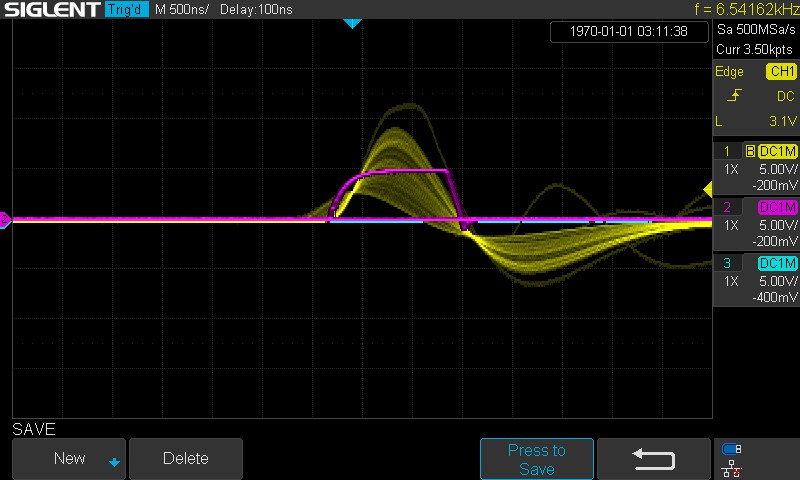
\includegraphics[width=1\textwidth]{../images/SDS00007.jpg}
	\end{center}
	\caption{CFD Spectrum for Moving Detector}\label{fig:sca_calib_m}
\end{figure}
\begin{figure}[H]
	\begin{center}
		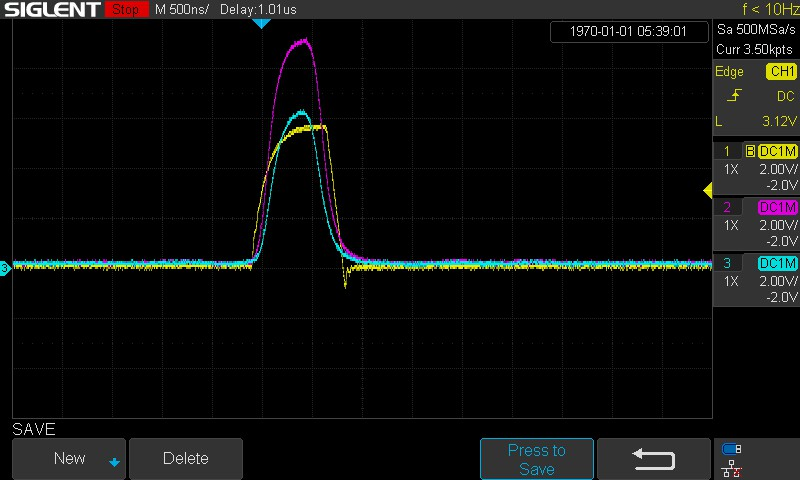
\includegraphics[width=1\textwidth]{../images/SDS00008.jpg}
	\end{center}
	\caption{CFD Spectrum for Moving Detector}\label{fig:sca_calib_m}
\end{figure}
\begin{figure}[H]
	\begin{center}
		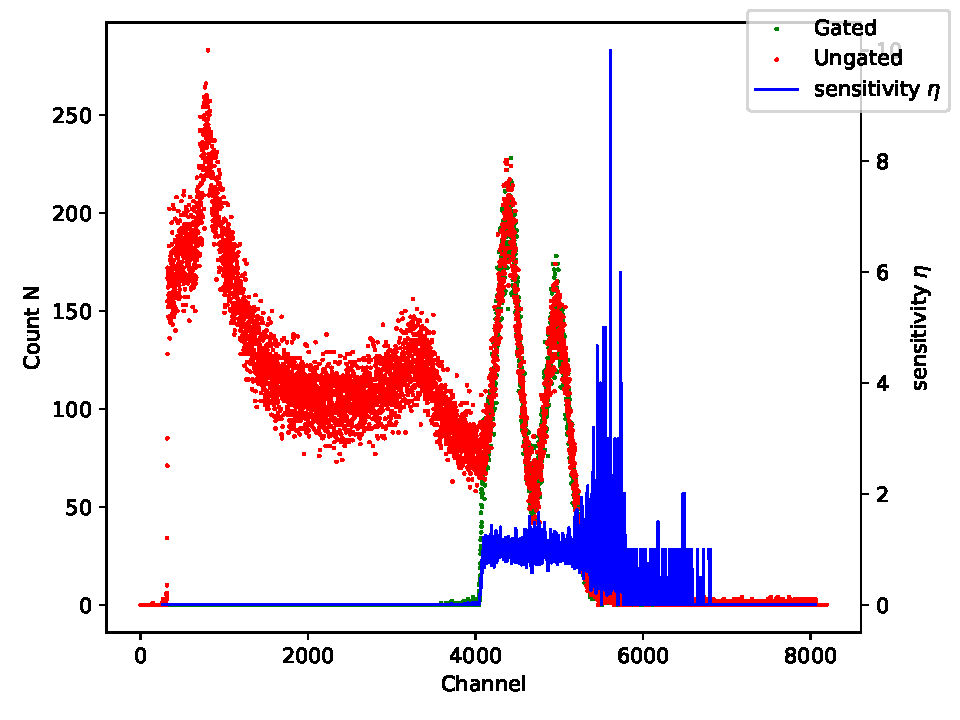
\includegraphics[width=1\textwidth]{../images/SCA_Calib.pdf}
	\end{center}
	\caption{CFD Spectrum for Moving Detector}\label{fig:sca_calib_m}
\end{figure}

\section{Main Analysis}
With the constructed circuit the random measurement and main measurement are taken. For the random measurements a total of 13 angles ranging from \SI{90}{\degree} to \SI{270}{\degree} in \SI{15}{\degree} steps are taken. At each angle the count coincidence rate is measured for 10 Minutes. Since the random measurement is done in 2 runs, every angles was measured twice. For the main measurement the total runs were increased from 2 to 6 and the measuring time per angles per run was increased from 10 Minutes to 12 Minutes.
\subsection{Random Measurements}
\subsubsection{Direct Measurement}\label{sec:dm}
To investigate the random coincidences of the signals, the delay in the fast branch is set to maximal difference to ensure no true coincidence is at play. Now only accidental overlapping signals trigger a coincidence. The rate of random coincidences can be determined by two methods. First, the gated counts are taken. Those already are the random coincidences since only when the signals of the fast branches overlap, a signal from the slow branch is received. As for all measured counts from the spectrum, a Poisson distribution is assumed, such that the uncertainty is
\begin{align}
	\sigma_N=\sqrt{N}
\end{align}
Suppose a count of 0 is registered. That would have yield an uncertainty of also 0. Since an uncertainty of zero is not realistic, a conservative correction is taken such that an uncertainty of
\begin{align}
	\sigma_N=\sqrt{N+1}
\end{align}
is assumed.
This yields the count rate distribution shown in \Cref{fig:dm}
\begin{figure}[H]
	\begin{center}
		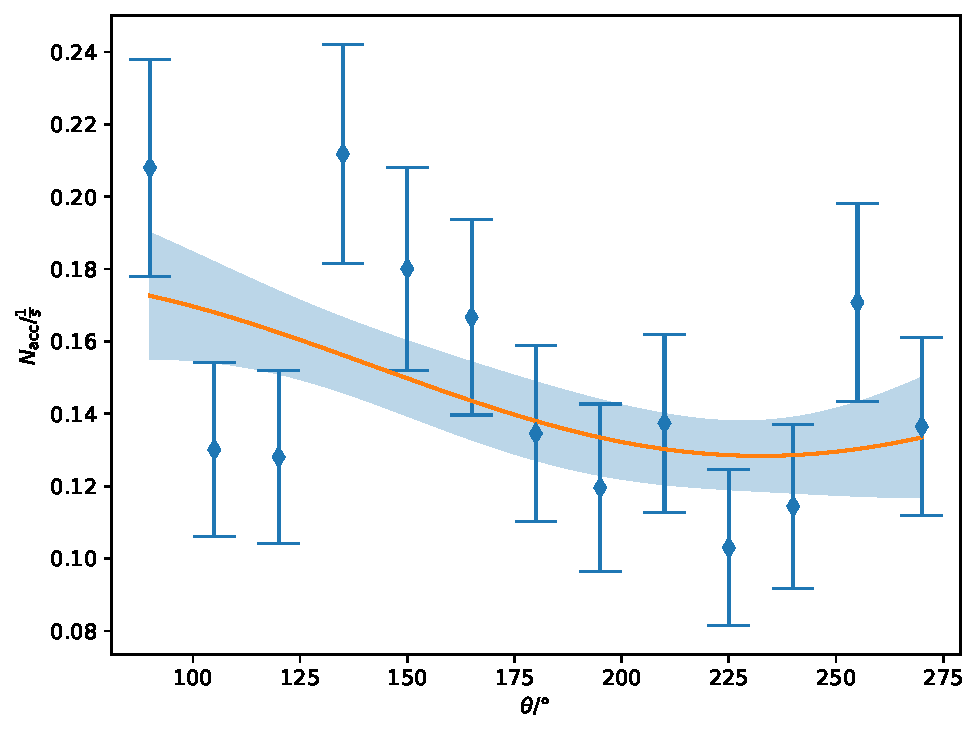
\includegraphics[width=1\textwidth]{../images/direct_measurement.pdf}
	\end{center}
	\caption{Direct Measurement of Random Coincidences from}\label{fig:dm}
\end{figure}
It can be seen that the distribution is anisotropic, i.e. specific directions increase the count-rate. This can be caused by strong radio active sources in the vicinity of the experiment apparatus. Therefore, the rate of random coincidences is dependent on the angle. The shown fit is of the form
\begin{align}
	N(\theta)=a+b\cdot\cos{\left(2\cdot\pi\frac{\theta}{360}-c\right)}\label{eq:nrand}
\end{align}
wtih paramters $a=\SI{0.153+-0.014}{}, b=\SI{-0.025+-0.015}{}$ and $c=\SI{110.87+-0.7}{}$ and has a quality of $\chi^2/\text{ddof}=1.57$, proving the function to be valid for modeling the distribution. Here it should be notice that $2\pi$ periodicity is enforced, since for a full rotation of the moving detector, the same signal is expected.
\subsubsection{Resolving Time and Single Detector Count Rates}
Another method is to calculate the accidental coincident rate with the resolving time and the count rate of the two detectors. For this the formula
\begin{align}
	N_\text{acc}=\sigma\cdot N_1\cdot N_2\text{\cite{leo1994techniques}}\label{eq:cos}
\end{align}
is used. Here we have the count rates $N$ and the resolving time $\sigma=2\tau$. The resolving time is set at the fast coincidence module to $\sigma=\SI{30+-4}{ns}$. The large uncertainty does not come from used modules, but represents the range of the resolving time such that the coincidence is reasonable.

The count rates are shown in \Crefrange{fig:cr1}{fig:cr2}
\begin{figure}[H]
	\begin{center}
		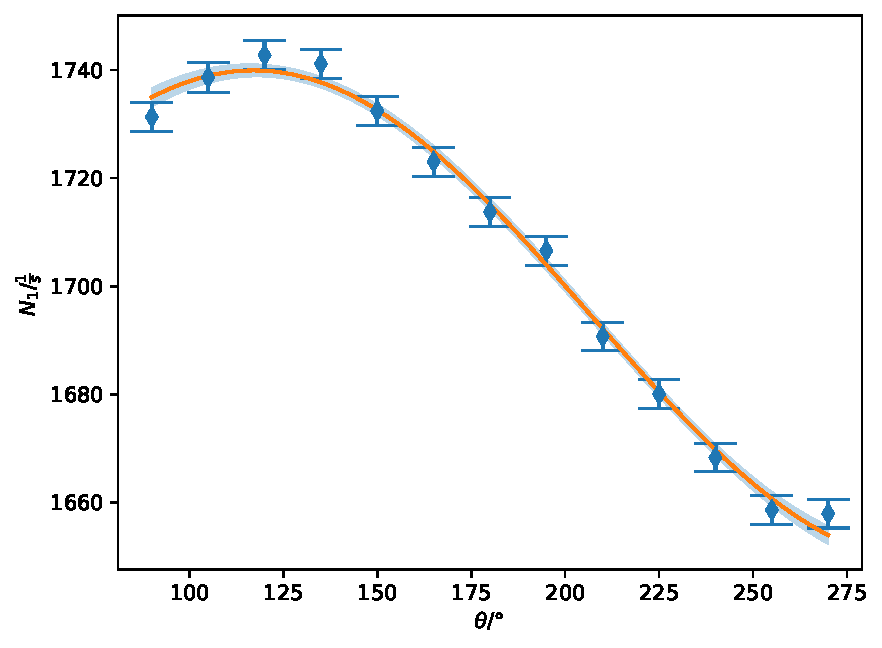
\includegraphics[width=1\textwidth]{../images/rnd_coinc_det_0.pdf}
	\end{center}
	\caption{Count Rate for Detector 1 (Moving)}\label{fig:cr1}
\end{figure}
\begin{figure}[H]
	\begin{center}
		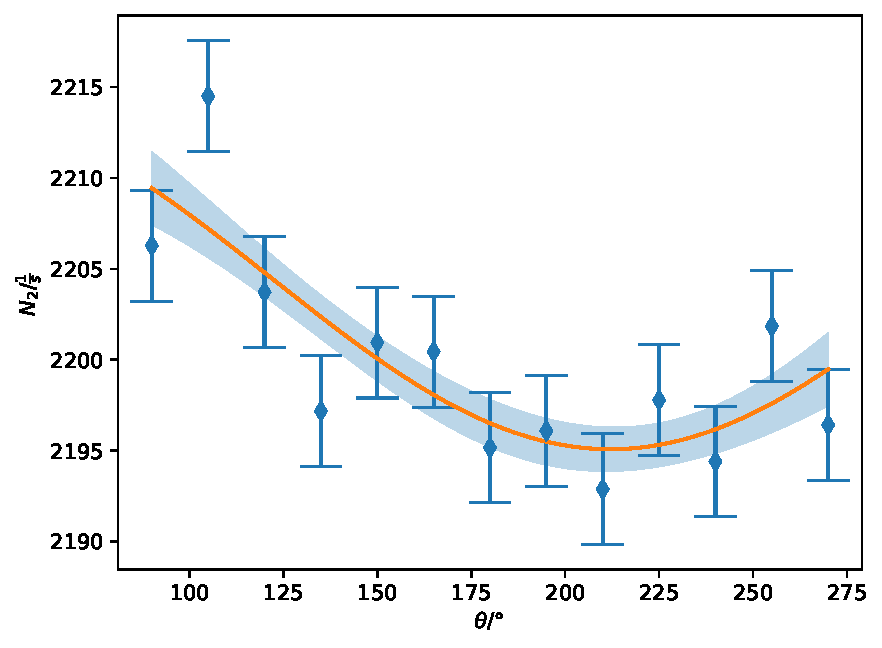
\includegraphics[width=1\textwidth]{../images/rnd_coinc_det_1.pdf}
	\end{center}
	\caption{Count Rate for Detector 2 (Stationary)}\label{fig:cr2}
\end{figure}
As seen before in the direct measurement, an anisotropic distribution is observed in the moving detector. The quality $\chi^2/\text{ddof}=\num{0.97}$ is well within a reasonable range with parameters $a=\SI{1694.4+-1.5}{}, b=\SI{45.5+-1.3}{}$ and $c=\SI{2.043+-0.043}{}$. Optimally the quality should be 1. On the other hand, the quality $\chi^2/\text{ddof}=\num{1.52}$ of the stationary detector is fairly high but also within a reasonable range wiht paramters $a=\SI{2204.5+-1.7}{}, b=\SI{9.4+-2.2}{}$ and $c=\SI{6.84+-0.17}{}$. Even though the stationary detector should not be dependent on the angle, a dependency is still assumed, since the moving detector can screen of certain parts of the field of view of the stationary detector and thus influence the count rate. Here is also a $2\pi$ periodicity assumed. Using the \Cref{eq:cos} again is probably not perfectly modeling the behaviour. A more appropriate Ansatz is an expansion in the spherical harmonics, where the data is fitted for the coefficients, since the spherical harmonics constitute a complete set. Taking another look at \Cref{eq:cos} one might notice, that this is in fact already a expansion to first order in $l$ and $m=0$ of the spherical harmonics. This and the fact that the quality is close to 1, justifies still using \Cref{eq:cos}.

As a result of the count rates and resolution \Cref{fig:crr} is obtained.
\begin{figure}[H]
	\begin{center}
		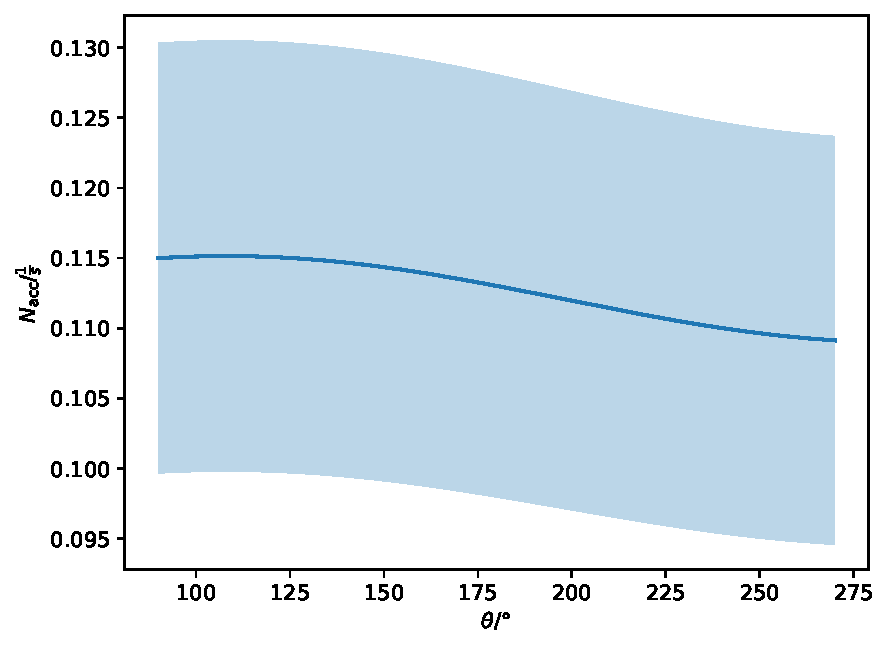
\includegraphics[width=1\textwidth]{../images/rnd_coinc_rate.pdf}
	\end{center}
	\caption{Accidental Coincidences Calculated through Resolving Time and Count Rates of Detector 1 and 2}\label{fig:crr}
\end{figure}
For this the functions for $N_1(\theta)$ and $N_2(\theta)$ are used. As seen a small dependency on the angle is present. More significant though, is the large uncertainty, here seen from the large confidence band colored blue. So no real information beyond Gaussian distribution can be assumed. Thus the weighted mean using the original data points for the count rates is computed to an average of $\bar{N}=\SI{0.1125+-0.0042}{\frac{1}{s}}$.

The calculated coincidence rate is with \SI{4.8}{\sigma} not very close to the directly measured accidental coincidence rate, which is ranging from \SI{0.133}{} to \SI{0.175}{} (see \Cref{fig:dm}). This deviation will stem from systematic errors, where the uncertainty on some measurements are underestimated or electronic noise could have triggered more coincidences in the fast branch, then would normally be triggered by external radiation that were originally planed to be measured by the random measurement.

\subsection{Stability Check}
To investigate the stability of the detectors over time, the main measurement is used to look at the fluctuations of the signals of the moving and stationary detector for constant angles over the multiple measurements for the different runs. Here fluctuations are defined as the standard deviation of of the signal over the different runs, since the runs happen at different points in time.

If the detectors would be stable over time, all fluctuations of the count rate would be within the uncertainty given by the Poisson distribution, i.e. the fluctuations could be caused by the uncertainty. Therefor at each angle the standard deviation and the uncertainty is calculated. Here the uncertainty is calculated as for every weighted mean like
\begin{align}
  \bar{\sigma}_x=\sqrt{\frac{1}{\sum_i\sigma_i^{-2}}}
\end{align}
To compare the different angles to each other, the standard deviation and the uncertainty are then divided by the mean of the count rates for each angle. This of course makes them only approximative comparable, but that should suffice for this analysis. As a result \Cref{fig:scd1} and \Cref{fig:scd2} are obtained for the moving detector and stationary detector respectively.
\begin{figure}[H]
	\begin{center}
		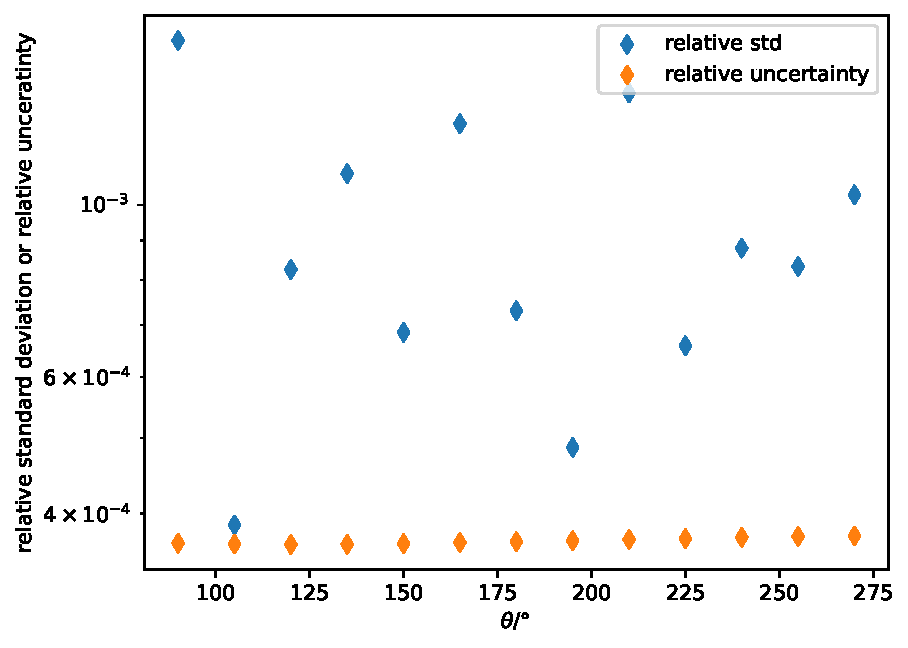
\includegraphics[width=1\textwidth]{../images/stab_count_det1.pdf}
	\end{center}
	\caption{Relative Standard Deviation and Uncertainties of Count Rates for Constant Angles of the Moving Detector}\label{fig:scd1}
\end{figure}
\begin{figure}[H]
	\begin{center}
		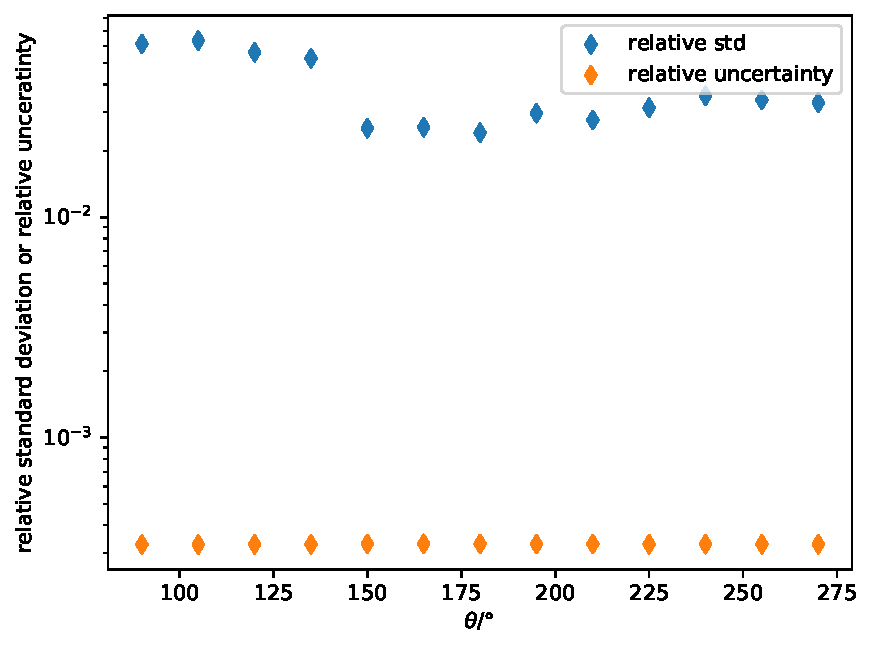
\includegraphics[width=1\textwidth]{../images/stab_count_det2.pdf}
	\end{center}
	\caption{Relative Standard Deviation and Uncertainties of Count Rates for Constant Angles of the Stationary Detector}\label{fig:scd2}
\end{figure}
For the moving detector and all angles, the fluctuation is higher then the uncertainty. The detector is not stable over time and the counts depend on the time measured. The same is the case for the stationary detector. Therefore the count rate is dependent on the specific time. To get more insight into the behaviour of the time dependency, the count rates are shown in \Crefrange{fig:scdb1}{fig:scdb2}. Here, over all runs are averaged. As always the weighted average is take, where the weight is the square of the inverse uncertainty.
\begin{figure}[H]
	\begin{center}
		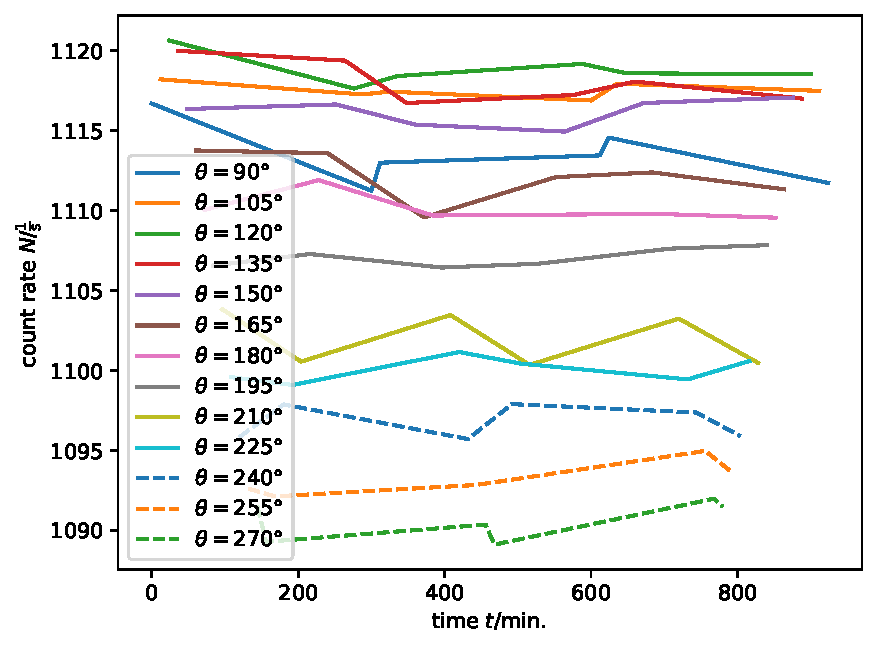
\includegraphics[width=1\textwidth]{../images/stab_count_det_behaviour_1.pdf}
	\end{center}
	\caption{Count Rates for Constant Angles of Moving Detector over Time}\label{fig:scdb1}
\end{figure}
\begin{figure}[H]
	\begin{center}
		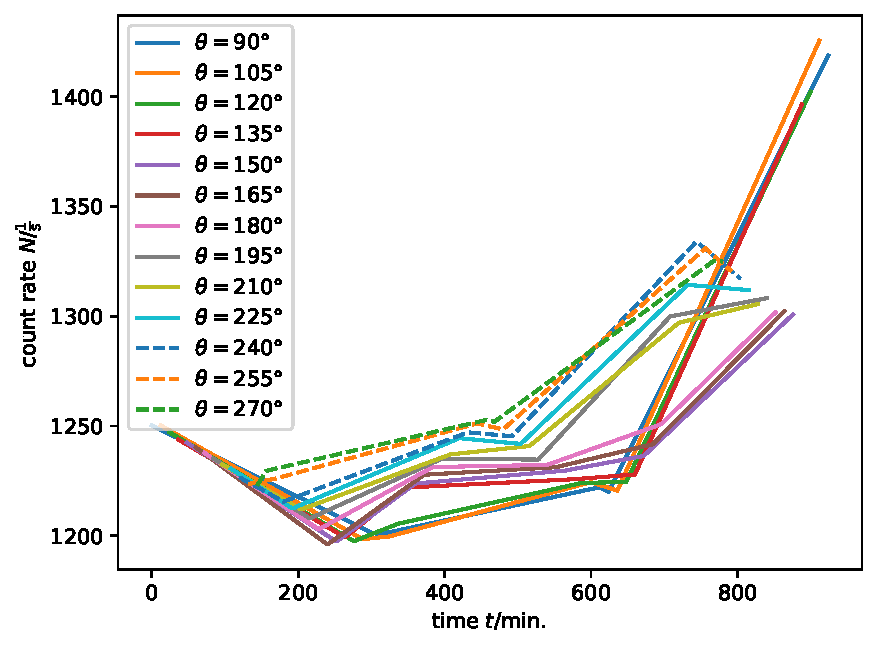
\includegraphics[width=1\textwidth]{../images/stab_count_det_behaviour_2.pdf}
	\end{center}
	\caption{Count Rates for Constant Angles of Stationary Detector over Time}\label{fig:scdb2}
\end{figure}
Against the usual manner, the data points are connected and uncertainties omitted. The purpose of this, is to enhance visibility for all 13 different angles, since only their general behaviour is of interest and not their exact values. From the figures themself it gets apparent that the count rate increases for all angles for the stationary detector, while this behaviour is even stronger for the first four angles. The moving detector has no such strong dependency on time.

The same procedure is now done with the total coincidence rate and with the fast branch coincidence rate instead of separating into detector 1 and 2, i.e. moving and stationary.
\begin{figure}[H]
	\begin{center}
		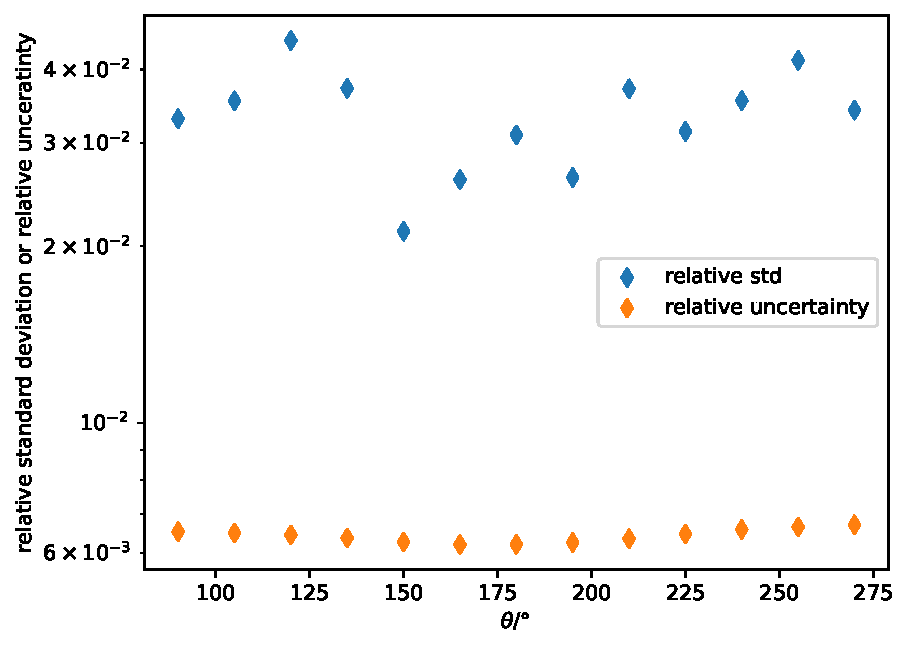
\includegraphics[width=1\textwidth]{../images/stab_count_circuit1.pdf}
	\end{center}
	\caption{Relative Standard Deviation of Count Rates for Constant Angles for the Coincidence Rate}\label{fig:scc1}
\end{figure}
\begin{figure}[H]
	\begin{center}
		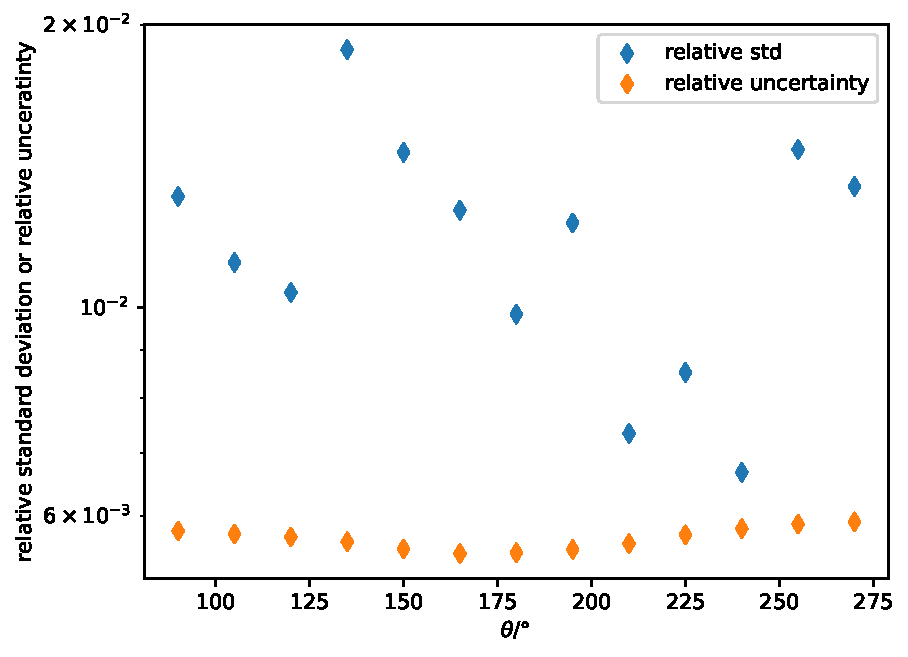
\includegraphics[width=1\textwidth]{../images/stab_count_circuit2.pdf}
	\end{center}
	\caption{Relative Standard Deviation of Count Rates for Constant Angles of the Fast Branch Coincidence Rate}\label{fig:scc2}
\end{figure}
All fluctuations are above the uncertainty (see \Crefrange{fig:scc1}{fig:scc2}), making them significant, i.e. non-neglectable. The count rates per angle over the measuring time are shown in \Crefrange{fig:sccb1}{fig:sccb2}.
\begin{figure}[H]
	\begin{center}
		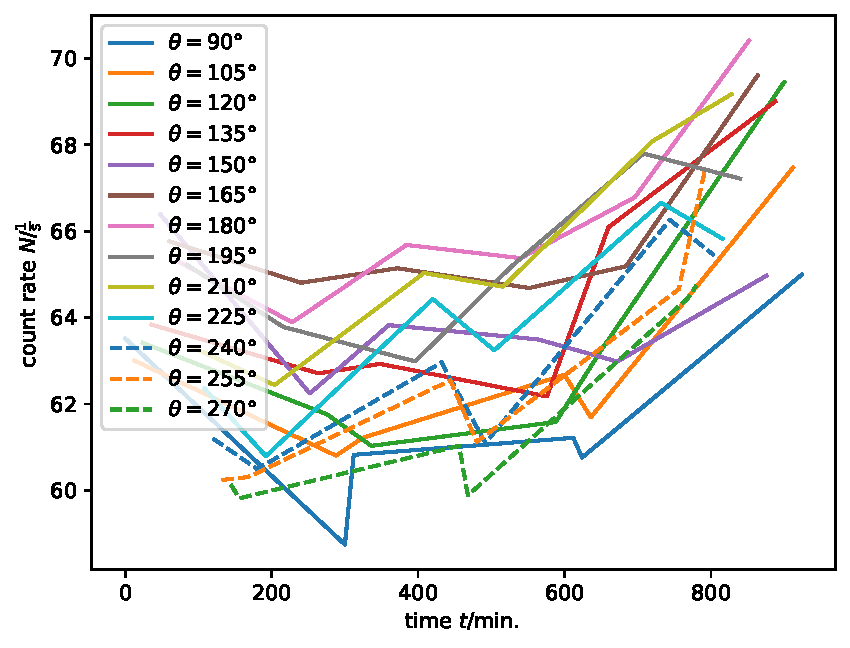
\includegraphics[width=1\textwidth]{../images/stab_count_circuit_behaviour_1.pdf}
	\end{center}
	\caption{Coincidence Rate for Constant Angles over Time}\label{fig:sccb1}
\end{figure}
\begin{figure}[H]
	\begin{center}
		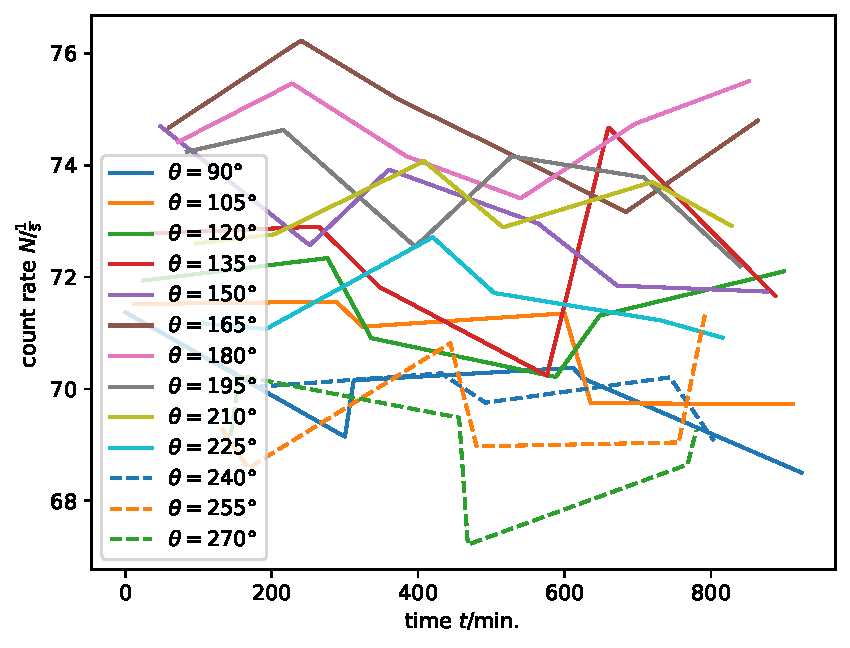
\includegraphics[width=1\textwidth]{../images/stab_count_circuit_behaviour_2.pdf}
	\end{center}
	\caption{Fast Branch Coincidence Rate for Constant Angles over Time}\label{fig:sccb2}
\end{figure}
The coincidence rate has a minimum around 300 minutes into the measurement for all angles, but increases again until the end to even higher coincidence rates then at the beginning of the measurement. The fast branch has no particular behaviour for the coincidence rates.

Overall, the time stability is poorly since the count rate is always dependent on the time when measured. Albeit this, the final result should not depend on this time dependency too strongly, since multiple measurements of the same angle are taken at different times, thereby should even out that time dependency.

To improve the measurement, it is advisable to make more runs and measure for less time per angle per run. For this measurement each angle was measured 12 minutes per run for a total of 6 runs and thus 936 minutes or 15 hours and 36 minutes. Doing e.g. 3 minutes per run for total of 24 runs would reduce the time dependency significantly, though taking the same amount. Of course the moving detector contributes a few extra seconds for repositioning but this should be neglectable. During the experiment the detector was noticed to take 2 to 4 seconds for moving.
\subsection{Correction for Random Coincidences}
From here on the random coincidences from the direct measurement in \Cref{sec:dm} are subtracted from the main measurement.
\subsection{Misalignment Correction}
Considering that the source is not perfectly centered, its misalignment is investigated. For this an angle dependent correction factor
\begin{align}
	\alpha(\theta)=\frac{N(\theta)}{N(180\degree)}
\end{align}
with
\begin{align}
	N(\theta; r_d, r_s, \theta_s)        & = \frac{N_0}{\Delta R(r_d, r_s, \theta, \theta_s)^2}, \\
	\Delta R(r_d, r_s, \theta, \theta_s) & =(\vec{R}(r_d, \theta)-\vec{R}(r_s, \theta_s))^2      \\
	\vec{R}(r, \theta)                   & =r\begin{pmatrix}
		                                         \cos\theta \\
		                                         \sin\theta \\
	                                         \end{pmatrix}
\end{align}
results in
\begin{align}
	\alpha(\theta)=\frac{r_d^2-2r_dr_s\cos{(180\degree - \theta_s)}+r_s^2}{r_d^2-2r_dr_s\cos{(\theta - \theta_s)}+r_s^2}
\end{align}
The main measurement data is used to show this ratio $\alpha$ in \Cref{fig:mis}
\begin{figure}[H]
	\begin{center}
		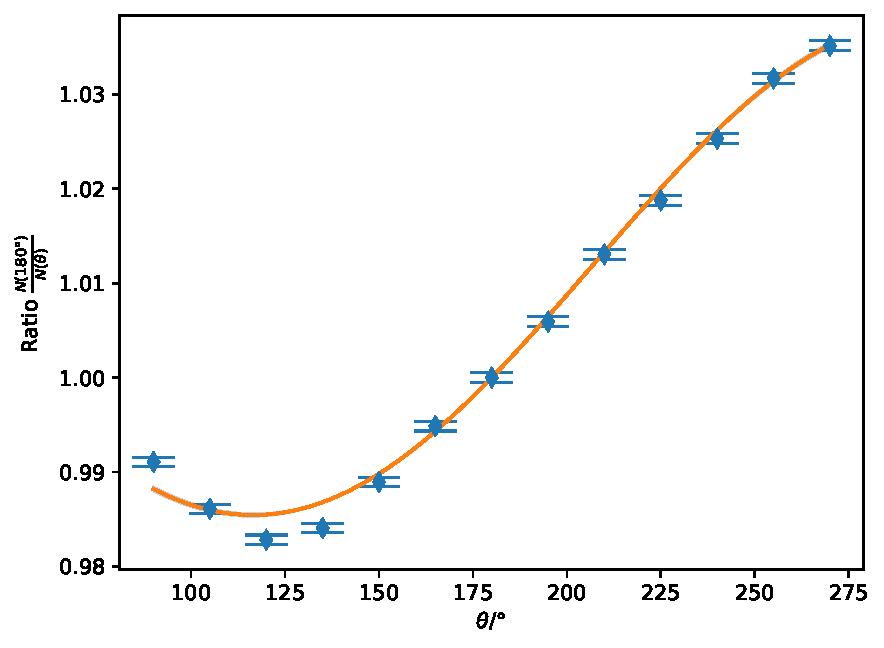
\includegraphics[width=1\textwidth]{../images/misal.pdf}
	\end{center}
	\caption{Misalignment Measurement}\label{fig:mis}
\end{figure}
As a result the displacement $r_s=\SI{64.9\pm1.3}{\mu m}$ at angle $\theta_s=\SI{116.5\pm1.4}{\degree}$ with a fit quality of $\chi^2/\text{ddof}=\num{9.82}$ is found. The $\chi^2$ is very high and shows that during the experiment and analysis larger systematic uncertainties have not been accounted for or wrong assumptions have been made, e.g. the movable detector is in fact not at the same distance and is not the exact same model as the stationary detector, changing the distance from the source.

This correction ratio $\alpha(\theta)$ can now be applied for the final analysis by multiplying the ratio with the count rates. It will correct of up to 4.5\% as seen in \Cref{fig:mis}.


\subsection{Solid Angle Corrections}
Since the detector is not point-like but has a spacial volume, the incoming rays are not perfectly normal to the detector surface. Therefore a correction has to be made to coefficients
\begin{align}
	A_{ii}=\frac{A_{ii}^\text{exp}}{Q_{ii}(r_1)Q_{ii}(r_2)}\label{eq:fds}
\end{align}
of the expansion of the angular correlation function
\begin{align}
	W(\theta)=N_0\cdot(1+A_{22}P_2(\cos\theta)+A_{44}P_4(\cos\theta))\label{eq:acf}
\end{align}
Since the in the previous section determined displacement of \SI{64.9\pm1.3}{\mu m} is within the uncertainty of \SI{1}{mm} of the authors ability to measure the distances, the source can be seen as centered. Additionally it is assumed that the detectors have the same distance to the source, \Cref{eq:fds} can be simplified with $r_1=r_2=r=\frac{d}{2}$ where $d=\SI{90+-1}{mm}$ is the distance from detector 1 to detector 2. Additionally it is assumed that the scintillator is \SI{5}{mm} deep into the detector, making the total distance $\SI{10+-1}{mm}$. Therefore the detectors are separated by \SI{5}{cm} from the source. Numerical values are given for the correction factors where they depend on this distance and the energy of the photon \cite{siegbahn}. Even though the observed transitions happen at \SI{1173.2}{keV} and \SI{1332.5}{keV}, the correction factors plateau beyond \SI{1}{MeV}. Thus the correction factors $Q_{22}(r)=\SI{0.9057}{}$ and $Q_{44}(r)=\SI{0.7113}{}$ for photons of \SI{1}{MeV} are used.

\subsection{Angular Correlation Function}
The count rates are now corrected by misalignment and random coincidences multiplying with the correction factor $\alpha(\theta)$ and subtracting the random coincidences
\begin{align}
	N_\text{corr}(\theta) = N(\theta)\cdot\alpha(\theta)-N_\text{rand}(\theta)
\end{align}
Here the random coincidence function $N_\text{rand}(\theta)$ corresponds to \Cref{eq:nrand} with the parameters from the direct measurement of the random coincidences. As a result the distribution in \Cref{fig:main} is obtained.
\begin{figure}[H]
	\begin{center}
		
\includegraphics[width=1\textwidth]{../images/main.pdf}
	\end{center}
	\caption{Main Measurement}\label{fig:main}
\end{figure}
Here the fit to the angular correlation function in \Cref{eq:acf} is done. The quality $\chi^2/\text{ddof}=\SI{0.22}{}$ with parameters $N_0=\SI{5.411+-0.011}{}$, $A_{22}^\text{exp}=\SI{0.0799+-0.0037}{}$ and $A_{44}^\text{exp}=\SI{0.0067+-0.0047}{}$ is achieved. With the correction from the previous section the coefficients are adjusted to $A_{22}=\SI{0.097+-0.013}{}$ and $A_{44}=\SI{0.0045+-0.0093}{}$. Given their large uncertainties, they lie within $1\sigma$ of the literature values $A_{22}^\text{lit}=\SI{0.1020}{}$ and $A_{44}^\text{lit}=\SI{0.0091}{}$ \cite{siegbahn}. Especially $A_{44}=\SI{0.0045+-0.0093}{}$ has an uncertainty larger then the value itself.

Last but not leas, other cascades are are fitted to the experimental distribution. The chosen cascades and the fit results are in \Cref{fig:maincas} with \Cref{tab:casc}. Here the coefficients $A_{ii}=F_i(L_1L_1I_iI)\cdot F_i(L_2L_2I_fI)$ for a $I_i(L_1)I(L_2)I_f$ cascade are set to literature values of the corresponding cascade\cite{siegbahn} and only the normalisation $N_0$ is optimized.
\begin{figure}[H]
	\begin{center}
		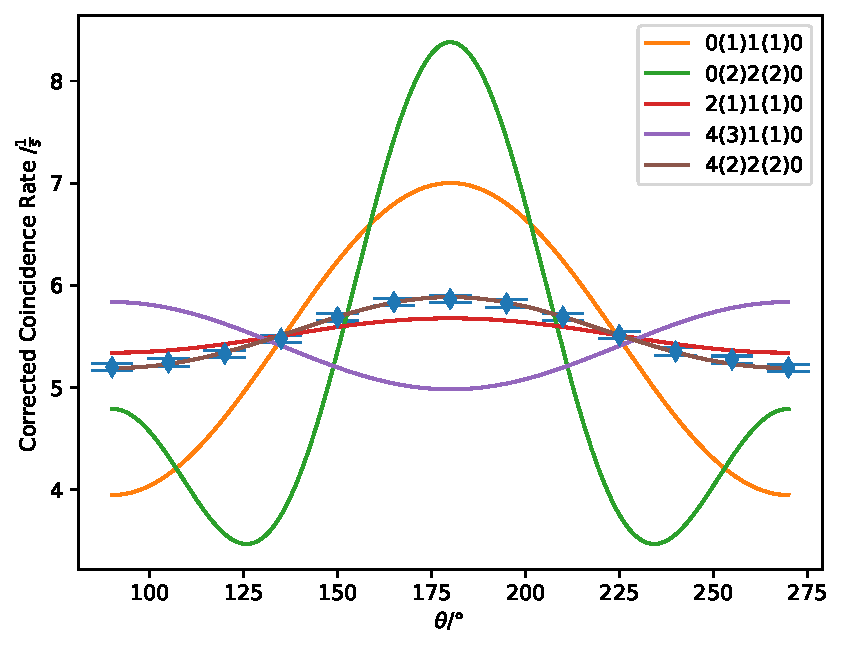
\includegraphics[width=1\textwidth]{../images/main_other.pdf}
	\end{center}
	\caption{Different Cascades Fitted to the Experimental Angular Distribution}\label{fig:maincas}
\end{figure}
\begin{table}
		\begin{tabular}{c|cc}
			cascade & $\chi^2/\text{ddof}$ & $N_0$                   \\
			\hline
			$0-1-0$ & $\num{657.31}$     & \SI{4.9661+-0.0092}{} \\
			$0-2-0$ & $\num{1647.61}$    & \SI{4.4778+-0.0084}{} \\
			$2-1-0$ & $\num{12.22}$      & \SI{5.4537+-0.0099}{} \\
			$4-1-0$ & $\num{255.81}$     & \SI{5.553+-0.01}{}    \\
			$4-2-0$ & $\num{0.28}$       & \SI{5.4087+-0.0098}{}
		\end{tabular}
		\caption{Quality for Normalisation Constant $N_0$ Fitted to Different Cascades}\label{tab:casc}
\end{table}
As seen, the assumed $4-2-0$ is most likely correct since the quality is here best, even though the $\chi^2$ is quite low, which shows, that more data is needed.

\section{Conclusion}
The experiment started by adjusting the different components for the final setup. For this the amplifier gain wa


After collection the data from the random and main measurement, the analysis started. For this the random coincidence rate was determined by directly measuring the coincidence (and by calculating it with the single count rates of the moving and stationary detector and the resolving time. A 





\bibliography{refs}
\end{document}
